\chapter{Hábitos e Práticas}

\begin{center}
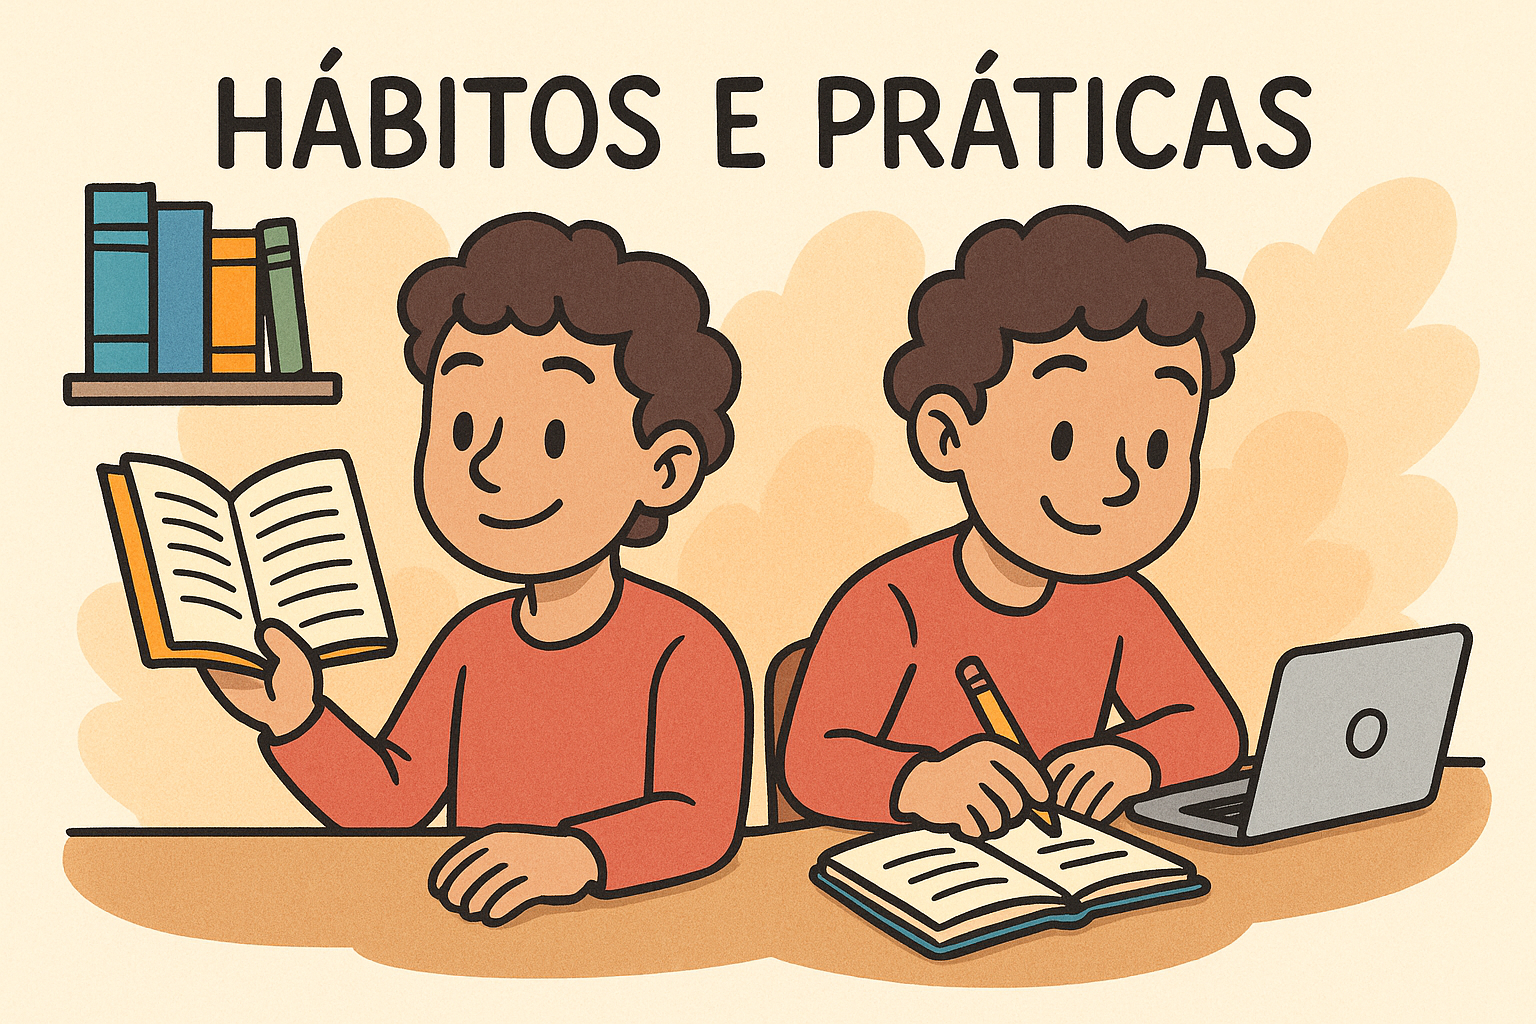
\includegraphics[width=0.5\linewidth]{Images/habitos.png}    
\end{center}
\vspace{0.5cm}

Ao ingressar em um programa de pós-graduação, o aluno deixa de ser apenas um receptor de conhecimentos e passa a atuar como um produtor de saberes. Esse processo exige o desenvolvimento de hábitos e práticas que sustentem uma formação científica sólida, crítica e produtiva. Neste capítulo, discutimos duas dessas práticas fundamentais: a leitura e a escrita.

Não se trata apenas de habilidades técnicas, mas de atitudes intelectuais que definem a postura do pesquisador diante do conhecimento. Ler é muito mais do que coletar informações — é construir um repertório teórico, compreender o estado da arte, dialogar com outros autores e localizar sua própria pesquisa dentro da comunidade científica. Escrever, por sua vez, é articular ideias com clareza, defender argumentos com coerência e contribuir para o avanço da ciência por meio da comunicação dos resultados.

Estes hábitos, quando cultivados com disciplina e intencionalidade, tornam-se ferramentas poderosas para a construção da autonomia acadêmica. O objetivo deste capítulo é apresentar orientações práticas para que o aluno desenvolva essas competências com consciência de sua importância e com estratégias que possam ser incorporadas à rotina de trabalho acadêmico.

\section{Deveres Éticos dos Alunos}

O aluno tem os seguintes deveres éticos

\begin{itemize}
      \item \textbf{Honestidade intelectual} – apresentar ideias e dados sem omissões ou distorções.
  \item \textbf{Originalidade e anti‑plágio} – citar corretamente todas as fontes, evitar auto‑plágio e uso indevido de IA generativa sem atribuição.
  \item \textbf{Responsabilidade na autoria} – incluir somente quem contribuiu de forma substancial e aceitar críticas construtivas.
  \item \textbf{Integridade de dados} – registrar e arquivar dados brutos; não manipular resultados para favorecer hipóteses.
  \item \textbf{Confidencialidade} – proteger informações sensíveis, respeitar acordos de sigilo e a Lei Geral de Proteção de Dados (LGPD).
  \item \textbf{Consentimento informado e bem‑estar de participantes} – obter aprovação do comitê de ética e garantir que participantes compreendam riscos e direitos.
  \item \textbf{Declaração de conflitos de interesse} – revelar laços financeiros, comerciais ou pessoais que possam influenciar o trabalho.
  \item \textbf{Uso responsável de recursos} – empregar laboratórios, equipamentos e verbas públicas ou privadas de modo eficiente e transparente.
  \item \textbf{Reprodutibilidade} – documentar metodologias, disponibilizar código e dados sempre que possível, facilitando a verificação por terceiros.
  \item \textbf{Profissionalismo e respeito} – tratar colegas, orientadores e participantes com civilidade, combater discriminação e assédio.
  \item \textbf{Conformidade institucional} – seguir regulamentos da universidade, agências de fomento e órgãos reguladores.
\end{itemize}




\needspace{5\baselineskip}
\section{A Prática da Leitura}


A leitura é a única forma do candidato a um título alcançar a maturidade necessária para defendê-lo. Muitos alunos têm uma boa ideia e acreditam que realizá-la e descrevê-la caracteriza uma tese. Isso não é verdade. 


\gxatencao{O aluno deve ler.}


Uma tese tem que ser colocada no contexto científico atual e comparada com os trabalhos já realizados sobre o assunto ou sobre temas similares ou análogos. Deve ficar claro, na tese, qual a colaboração que o trabalho traz à ciência. Obviamente, só é possível fazer isso se o aluno tiver um conhecimento da área, que deve ser, na maior parte das vezes, até mesmo superior ao conhecimento do orientador.


Quando o aluno não lê o suficiente isso fica muito claro para o orientador. Há uma falta de capacidade de argumentação, uma falta de base teórica para o trabalho. Um dos principais sinais de maturidade que um orientador percebe é a capacidade de argumentação baseada em evidências científicas.


É importante notar que não basta ler, mas é necessário ler publicações atualizadas (além dos textos clássicos da área).


Se você achar que está lendo pouco, ou se seu orientador reclamar disso, aqui estão algumas dicas:

\begin{outline}	
\1	Levante uma lista de congressos e revistas relativas à área de sua tese.
\2	Faça um mix com o máximo possível de publicações da área específica com publicações importantes da área mais geral.
\1	Obtenha os últimos cinco anos desses congressos e revistas.
\1	Liste todos os artigos disponíveis que possam servir para sua tese.
\1	Obtenha esses artigos.
\1	Leia os resumos e os organize de alguma forma, priorizando a leitura.
\2	Procure tutoriais e reviews para o início da leitura.
\2	Leia alguns artigos clássicos citados nos artigos obtidos.
\2 Leia os artigos específicos, com foco nos mais atuais.
\1	Mantenha o controle dessa lista e faça o acompanhamento com o orientador.
\end{outline}

A maioria dos textos de metodologia científica recomenda o fichamento dos artigos lidos. Essa prática é importante, porém não é mais necessário usar fichas. Você pode usar um banco de dados, um sistema de referência ou até mesmo um ou mais arquivos de documento, como arquivos Word. Até mesmo “Post-it” pode gerar um bom sistema de fichamento. 

A principal recomendação é sempre ler: Leia muito. Leia artigos sobre a teoria e sobre a aplicação. Leia revistas correlatas. Leia o jornal diariamente. Leia revistas de divulgação científica relacionadas ao seu trabalho. Leia revistas importantes nacionais e internacionais. A leitura é um hábito importante e deve ser desenvolvido constantemente. Leve todos os artigos interessantes para seu orientador ver. Se forem muito interessantes, leve uma cópia para deixar com ele. Desenvolva o hábito de trabalhar com seu orientador. 


\needspace{5\baselineskip}
\subsection{O aluno que só lê português (e não conta ao orientador)}


Dificilmente você será aceito no mestrado se sua capacitação em inglês não permite uma leitura em ritmo razoável, porém isso pode acontecer.


Nesse caso, deixe bem claro ao orientador sua dificuldade. Esconder qualquer dificuldade de leitura ou compreensão, seja ela de inglês ou de alguma matéria específica, fará com que seu orientador avalie sua dificuldade como falta de dedicação.


O resultado é que, em vez de o orientador ajudá-lo nessa dificuldade, ele tornará as coisas cada vez mais difíceis.


Por sinal, se esse for seu caso, entre imediatamente em um curso de inglês. Qualquer melhoria, junto com a leitura de textos da área, implicará em um rendimento maior do seu trabalho. Existem cursos gratuitos ou muito baratos na universidade.

\needspace{5\baselineskip}
\section{A Necessidade da Escrita}


É quase impossível seguir uma carreira acadêmica em qualquer área de sem escrever bem, pelo menos em português. 


Se você acha que escreve mal, ou se os outros acham que escreve mal, tente corrigir o mais rápido possível. Faça cursos e se esforce. Muitos alunos simplesmente acham “normal” um profissional de área técnica escrever mal. Isso demonstra uma falta de compreensão das necessidades do mundo real: apresentar e defender, de forma clara, suas ideias. 


Como diria o Chacrinha\footnote{É provável que alguns dos leitores mais novos não tenham conhecido o “Chacrinha”. Ele foi por muitos anos um apresentador de programa de auditório de muito sucesso, usando uma fantasia e utilizando bordões engraçados. Certamente foi uma das figuras mais conhecidas na TV brasileira do século XX.}: 


\gxatencao{Quem não se comunica, se trumbica}


Uma das principais indicações da educação de uma pessoa é sua capacidade de se expressar em sua língua mãe.


Ao estudante universitário, essa característica é muito desejada. Ao aluno de mestrado e doutorado, é indispensável.


Contribuição de um aluno que aprendeu a escrever.

\begin{quote}

Só consegue escrever quem consegue dizer o que pensa e quer.  Fale, diga o que pensa, conte para seu orientador suas ideias e busque clareza ao dizer.

Escreva simples.  Uma tese é, antes de qualquer coisa, uma coleção de folhas de papel com um monte de letrinhas em cima.  

Ler é, depois de falar, uma das melhores ajudas para quem quer aprender a escrever.  Ler tudo, de jornal a bula de remédio, passando por contos, poesias, história em quadrinhos, artigos e, naturalmente, uma tese ou outra de vez em quando.

Depois fica-se assim, querendo escrever em qualquer lugar, em qualquer oportunidade, em qualquer Wiki que se abra.

Desejo boa sorte a nós todos.

\textit{Bebeto}

\end{quote}

Uma das coisas mais importantes é estar em dia com a literatura da área. Isso significa que você tem que visitar pelo uma vez por mês cada site que possa ser útil para você, procurando publicações novas. Essa visita, hoje em dia, é virtual, normalmente por meio do Portal de Periódicos da CAPES mas nunca subestime a capacidade que temos de ter ideias folheando uma revista ou livro. 
Ou seja, não confie apenas na busca, mas também leia ou folheie as revistas científicas.

\gxatencao{Use o portal da Capes em http://www.periodicos.capes.gov.br/.}

\section{Gerenciando as Informações da Tese}

\subsection{O caderno de ´pesquisa}

Uma prática que dá muito certo é os alunos manterem um caderno normal, de papel mesmo, como registro de trabalho e reuniões.
Cadernos de pesquisa (ou de laboratório) são uma prática antiga que funciona. Recomendo fortemente.


Tenha sempre o caderno ao conversar com o orientador. Anote no caderno tudo que você fez, tudo que vai fazer.

Sei que muitos pensam em fazer isso digitalmente. Não é prático, pois não pode desenhar ou rabiscar no celular com a facilidade que faz no caderno.

Também são ótimos para criatividade e para guardar ideias que saem do nada. Algumas pessoas usam um caderno pequeno e mantém consigo o tempo todo.

Eu gosto de usar cadernos de folha branca ou quadriculada.

\subsection{A gestão das referências}

Use um software de controle bibliográfico. Existem vários no mercado, alguns gratuitos. Eu aconselho o Zotero, que é gratuito e funciona em rede\footnote{Zotero é adotado pela linha de Engenharia de Dados e Conhecimento e compartilhamos as referências por ele}. Outro bom software gratuito é o Mendeley. Os usuários de LaTeX podem usar o JabRef.

Anote tudo que ler. 
Faça fichamento e se possível coloque no software de controle bibliográfico. 
Porém, cuidado para o fichamento não ser inútil, use-o de maneira sensata.
O ideal é que você não tenha que ler nada duas vezes (a não ser na primeira vez, que pode na verdade exigir várias leituras). 
Mantenha o resumo de tudo. 

\subsection{O método Zettelkasten}

Criado pelo sociólogo alemão Niklas Luhmann, o \emph{Zettelkasten} (em alemão, “caixa de fichas”) define um sistema de gestão de conhecimento em que cada ideia é registrada em uma nota atômica, numerada de forma única e intencionalmente conectada a outras notas\citep{fast2020zettelkasten}.  

Os quatro princípios fundamentais são: 
\begin{enumerate}
    \item notas atômicas; 
    \item identificação única; 
    \item ligações bidirecionais, e 
    \item crescimento emergente da rede.  
\end{enumerate}

Essa estrutura transformaria o repositório em um ``segundo cérebro'' navegável, favorecendo \textit{insights} e escrita acadêmica de longo prazo.

\subsubsection{Fluxo de trabalho recomendado}

\begin{enumerate}
  \item \textbf{Fleeting note}: registe a ideia bruta em uma nota diária.  
  \item \textbf{Literature note}: extraia trechos relevantes de artigos ou livros, com referência completa.  
  \item \textbf{Permanent note}: destile o conceito em uma nota independente, atribua um ID cronológico (ex.: \texttt{20250713‑2359}), adicione links para notas relacionadas e, se necessário, \emph{tags}.  
  \item \textbf{Mapa de estrutura}: crie notas‑hub que agrupem e resumam subconjuntos temáticos, servindo de rascunho para capítulos ou artigos.
\end{enumerate}

Diversos programas, como Obsidian e Zettler, adotam o paradigma de Luhmann, oferecendo recursos de hiperligações, grafos e extensões de automação. 

Obsidian é um editor \emph{local‑first} baseado em Markdown que armazena todas as notas em arquivos‑texto simples\citep{obsidianGraphView}.  
Ligação reversa, painel de “links não citados”, \emph{graph view} interativo e um ecossistema de \emph{plug‑ins} (como \texttt{Citations}, \texttt{Dataview} e \texttt{Zettelkasten Prefixer}) tornam‑no uma escolha popular entre pesquisadores.

Zettlr é um editor Markdown \emph{open‑source} voltado para pesquisa acadêmica, com integração nativa a Pandoc e gerenciadores de referências BibLaTeX.  
Sua abordagem minimalista respeita o conceito de notas atômicas e IDs cronológicos, enquanto provê painel de estatísticas e busca em tempo real\citep{zettlrGuide}.



\subsubsection{Boas práticas}

\begin{enumerate}
  \item Use IDs cronológicos legíveis para evitar colisões.  
  \item Mantenha notas verdadeiramente atômicas; se puder ser citada isoladamente, merece arquivo próprio.  
  \item Revise semanalmente para “jardinar” links órfãos e dividir ou fundir fichas quando necessário.  
  \item Prefira ligações contextuais a listas extensas de \emph{tags}.  
  \item Publique ou exporte via Pandoc quando o conjunto de notas se consolidar em produto final (artigo, capítulo, relatório).
\end{enumerate}


